%iffalse
\let\negmedspace\undefined
\let\negthickspace\undefined
\documentclass[journal,12pt,onecolumn]{IEEEtran}
\usepackage{cite}
\usepackage{amsmath,amssymb,amsfonts,amsthm}
\usepackage{algorithmic}
\usepackage{graphicx}
\usepackage{textcomp}
\usepackage{xcolor}
\usepackage{txfonts}
\usepackage{listings}
\usepackage{enumitem}
\usepackage{mathtools}
\usepackage{gensymb}
\usepackage{comment}
\usepackage[breaklinks=true]{hyperref}
\usepackage{tkz-euclide} 
\usepackage{listings}
\usepackage{gvv}                                        
%\def\inputGnumericTable{}                                 
\usepackage[latin1]{inputenc}     
\usepackage{xparse}
\usepackage{color}                                            
\usepackage{array}                                            
\usepackage{longtable}                                       
\usepackage{calc}                                             
\usepackage{multirow}
\usepackage{multicol}
\usepackage{hhline}                                           
\usepackage{ifthen}                                           
\usepackage{lscape}
\usepackage{tabularx}
\usepackage{array}
\usepackage{float}
\newtheorem{theorem}{Theorem}[section]
\newtheorem{problem}{Problem}
\newtheorem{proposition}{Proposition}[section]
\newtheorem{lemma}{Lemma}[section]
\newtheorem{corollary}[theorem]{Corollary}
\newtheorem{example}{Example}[section]
\newtheorem{definition}[problem]{Definition}
\newcommand{\BEQA}{\begin{eqnarray}}
\newcommand{\EEQA}{\end{eqnarray}}
\usepackage{float}
\usepackage{listings}
\usepackage{xcolor}
%\newcommand{\define}{\stackrel{\triangle}{=}}
\theoremstyle{remark}
\usepackage{ circuitikz }
%\newtheorem{rem}{Remark}
% Marks the beginning of the document
\begin{document}
\title{10.3.2.5}
\author{EE24BTECH11007 - Arnav Makarand Yadnopavit}
\maketitle
\renewcommand{\thefigure}{\theenumi}
\renewcommand{\thetable}{\theenumi}
\parindent 0px Question: Half the perimeter of a rectangular garden, whose length is 4 m more than its width, is
36 m. Find the dimensions of the garden.\\
\solution\\
Let length and width of the garden be $x$ and $y$ respectively 
\begin{align}
    x+y=36\\
    x-y=4
\end{align}

We represent the system in matrix form:
\begin{align}
A = \myvec{1 & 1 \\ 1 & -1}, \quad
b = \myvec{36 \\ 4}, \quad
x = \myvec{x \\ y}.
\end{align}

\subsection*{$LU$ Decomposition of $A$}
We aim to decompose $A$ into $LU$, where:
\begin{align}
L = \myvec{1 & 0 \\ l_{21} & 1}, \quad
U = \myvec{u_{11} & u_{12} \\ 0 & u_{22}}.
\end{align}

Substituting $LU = A$:
\begin{align}
\myvec{1 & 0 \\ l_{21} & 1}
\myvec{u_{11} & u_{12} \\ 0 & u_{22}}
=
\myvec{1 & 1 \\ 1 & -1}.
\end{align}

From this:
\begin{align}
u_{11} &= 1, \quad u_{12} = 1, \\
l_{21}u_{11} &= 1 \implies l_{21} = 1, \\
l_{21}u_{12} + u_{22} &= -1 \implies 1(1) + u_{22} = -1 \implies u_{22} = -2.
\end{align}

Thus:
\begin{align}
L = \myvec{1 & 0 \\ 1 & 1}, \quad
U = \myvec{1 & 1 \\ 0 & -2}.
\end{align}

\subsection*{Solving $A{x} = {b}$}

\subsubsection*{Forward Substitution: Solve $Ly = b$}
\begin{align}
\myvec{1 & 0 \\ 1 & 1}
\myvec{y_1 \\ y_2}
=
\myvec{36 \\ 4}.
\end{align}

From the first row:
\begin{align}
y_1 = 36.
\end{align}

From the second row:
\begin{align}
y_1 + y_2 &= 4 \\
36 + y_2 &= 4 \\
y_2 &= -32.
\end{align}

Thus:
\begin{align}
{y} = \myvec{36 \\ -32}.
\end{align}

\subsubsection*{Back Substitution: Solve $Ux = y$}
\begin{align}
\myvec{1 & 1 \\ 0 & -2}
\myvec{x \\ y}
=
\myvec{36 \\ -32}.
\end{align}

From the first row:
\begin{align}
x + y = 36.
\end{align}

From the second row:
\begin{align}
-2y = -32 \\
y = 16.
\end{align}

Substitute $y = 16$ into the first equation:
\begin{align}
x + 16 = 36 \\
x = 20.
\end{align}

Thus:
\begin{align}
x = 20, \quad y = 16.
\end{align}





\begin{figure}[H]
    \centering
    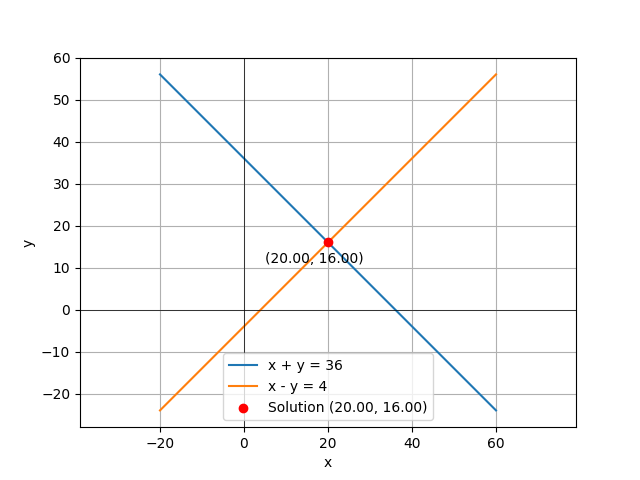
\includegraphics[width=\columnwidth]{figs/fig.png}
 \end{figure}
\end{document}


